\documentclass[9pt]{beamer}

\usepackage[brazilian]{babel}
\usepackage[utf8]{inputenc}
\usepackage[T1]{fontenc}
\usepackage{beamerthemesplit}
\usepackage{advdate}

\graphicspath{ {imagens/} }

\title{Utilização de Redes Neurais Recorrentes Para Predição de Controle de Estoque}

\author{Eduardo Rodrigues de Faria Filho  \\ \and Gabriel Augusto De Vito D'Abbadia Guimarães }
\institute{Professor Orientador: Sandrerley de Ramos Pires \\  Universidade Federal de Goiás}
\date{\today}
\setbeamertemplate{caption}[numbered]

\begin{document}
	\frame{\titlepage}
	
	\section{Sumário}
	\frame
	{
		\frametitle{Sumário}
		
		\textbf{Tópicos}
		
		\begin{enumerate}
			\item Introdução
			\begin{enumerate}
				\item O Problema
				\item Objeto de Estudo
				\item Justificativa
				\item Objetivos
				\begin{enumerate}
					\item Objetivo Geral
					\item Objetivos Específicos
				\end{enumerate}
				\item Metodologia e Cronograma de Atividades
			\end{enumerate}
			\item Referencial Teórico
			\begin{enumerate}
				\item Redes Neurais Recorrentes
			\end{enumerate}
			
		\end{enumerate}
	}


	\section{Introdução}
		
		\subsection{Introdução}
			\frame {
				\frametitle{Introdução}
				\begin{itemize}
					\item{Necessidade de aprimorar o controle de estoque da empresa;}
					\item{Necessidade da informação para uma melhor tomada de decisão;}
					
					\begin{figure}[h!]
						\centering
						\caption{Campinorte}
						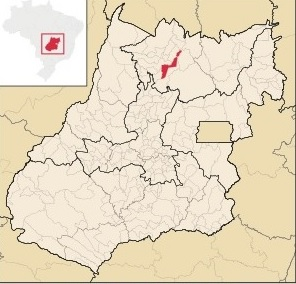
\includegraphics[scale=0.25]{campinorte.jpg}
						\\
						\footnotesize Fonte: Campinorte - Wikipedia, a enciclopédia livre. 16 nov. 2018. Disponivel em: <https://pt.wikipedia.org/wiki/Campinorte/>. Acesso em: 09 dez. 2018.
					\end{figure}	
				
				\end{itemize}
				
			}	
		
		
			\frame {
				\frametitle{Introdução}
				\begin{itemize}
					\item{Armazenar somente o necessário para o período de vendas;}
					\item{Utilização de redes neurais recorrentes para solucionar o problema;}
				\end{itemize}
			
				\begin{figure}[h!]
					\centering
					\caption{Exemplo de armazenamento de milho debulhado em sacos}
					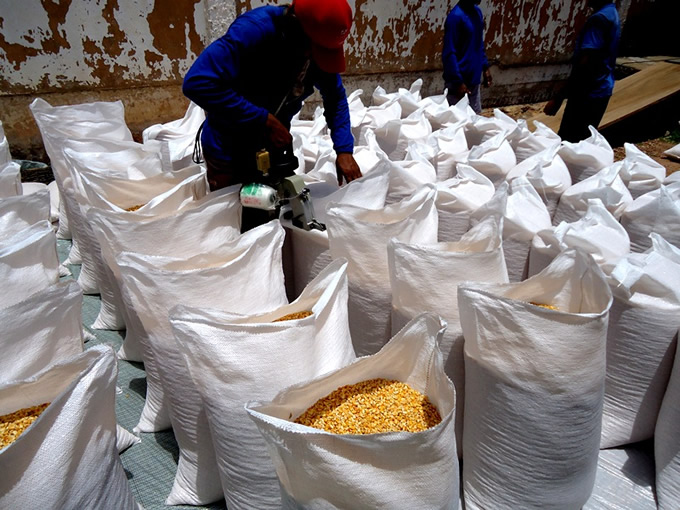
\includegraphics[scale=0.15]{milho.jpg}
					\\
					
					\footnotesize Fonte: Conab vai adquirir 28 mil toneladas de milho ensacado para PB e RN, 14 mai. 2013. Disponivel em: <https://www.paraibainforma.com.br/conab-vai-adquirir-28-mil-toneladas-de-milho-ensacado-para-pb-e-rn/>. Acesso em: 09 dez. 2018.
				
					
				\end{figure}		
			}
			
			
		\subsection{O Problema}	
			\frame {
				\frametitle{O Problema}
				
				\begin{itemize}
					\item{No Brasil, de acordo com Confederação Nacional do Comércio 30,7\% das lojas tinham estoques acima do apropriado e 14,3\% abaixo do apropriado;}
					\item{Dados do (SEBRAE, 2014) apontam que 50\% das empresas que fecharam no período da pesquisa não definiram estratégias para evitar desperdícios;}
					\item{Melhorar o controle de estoque e consequentemente a gestão da empresa;}
					\item{Se posicionar melhor no mercado comparado aos concorrentes;}
					\item{Evitar má reputação com os clientes;}
					
				\end{itemize}
			}
		
		
		\subsection{Objeto de Estudo}
			\frame {
				\frametitle{Objeto de Estudo}
				\begin{itemize}
					\item{Série temporal dos dados de venda do milho debulhado;}
					\item{Refinamento do problema e construção da solução analisando fatores externos a empresa;}
				\end{itemize}
					\begin{figure}[h!]
						\centering
						\caption{Exemplo de uma série temporal de vendas de milho debulhado (exemplo fictício)}
						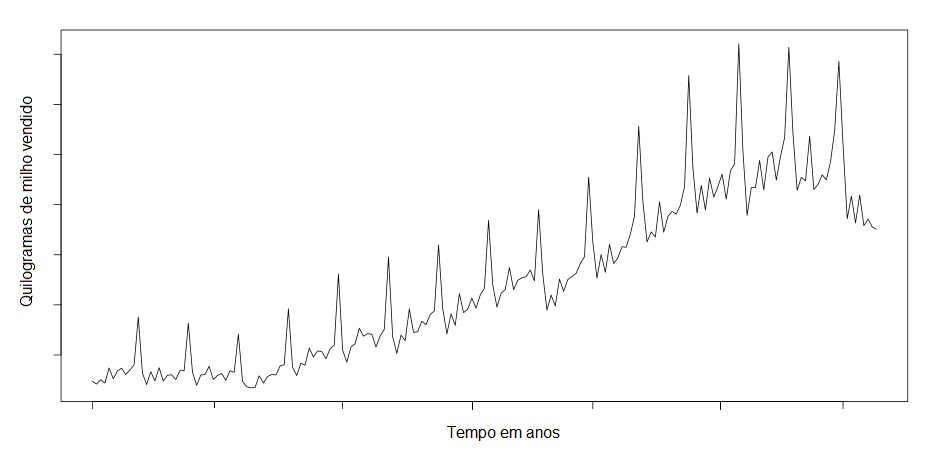
\includegraphics[scale=0.3]{serie.jpeg}
						\\
					\footnotesize Fonte: Próprio autor
					\end{figure}
			}
		
		
		\subsection{Justificativa}
			\frame {
				\frametitle{Justificativa}
				\begin{itemize}
					\item{Avanços significativos na área beneficiando toda a sociedade;}
					\item{Utilização em ambientes corporativos;}
					\item{Uso e estudo de redes neurais recorrentes para resolver problemas de séries temporais como a do problema;}
				\end{itemize}
			}
		
		
		\subsection{Objetivo Geral}
			\frame {
				\frametitle{Objetivo Geral}
					
		 		Utilizando uma ferramenta de predição, baseada em inteligência artificial, prever a demanda de venda de milho debulhado que é comercializado pela empresa atendida neste trabalho;	 	
				
			}
		
		\subsection{Objetivos Específicos}
			\frame {
				\frametitle {Objetivos Específicos}	
				
					\begin{enumerate}
						\item Revisão Bibliográfica Sistemática sobre redes neurais recorrentes;
						\item Identificar e capturar dados sobre os elementos internos e externos que possam influênciar na demanda de milho debulhado;
						\item Elaborar um algoritmo que seja capaz de relacionar os dados históricos (tanto de fatores externos quanto de vendas) da empresa, capaz de predizer a quantidade ideal que ela deve ter em estoque em um determinado período;
						\item Realizar um comparativo gráfico entre os valores obtidos e valores reais;
					\end{enumerate}	
			}
		
		
		\subsection{Metodologia e Cronograma de Atividades}
			
		
			\frame {
				\frametitle{Metodologia e Cronograma de Atividades}
				\begin{figure}[h!]
					\centering
					\caption{Cronograma de Atividades}
					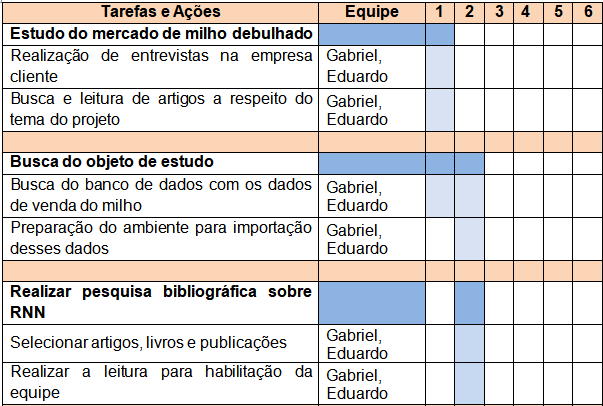
\includegraphics[scale=0.4]{metodologia.png}
					\\
				\footnotesize Fonte: Próprio autor
				\end{figure}
			}
		
			\frame {
				\frametitle{Metodologia e Cronograma de Atividades}
				\begin{figure}[h!]
					\centering
					\caption{Cronograma de Atividades}
					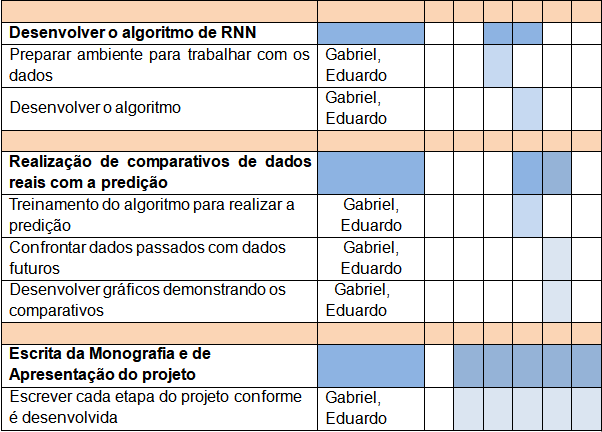
\includegraphics[scale=0.4]{metodologia2.png}
					\\
					\footnotesize Fonte: Próprio autor
				\end{figure}
			}
		
		
	\section{Referencial Teórico}
		\subsection{Redes Neurais Recorrentes}
		\frame {
			\frametitle{Redes Neurais Recorrentes}
			\begin{figure}[h!]
				\centering
				\caption{Comportamento de Redes Neurais Recorrentes}
				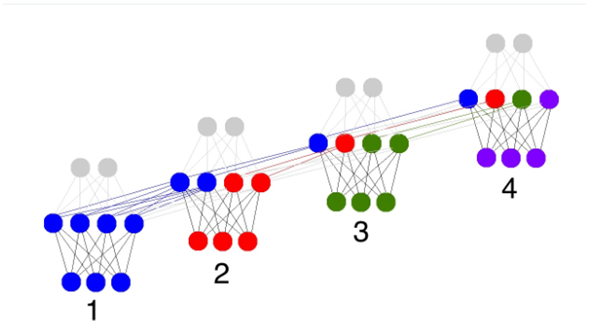
\includegraphics[scale=0.4]{rnn.png}
				\\
				\footnotesize Fonte: UM mergulho profundo nas redes neurais recorrentes. iMasters, 05 set. 2017. Disponivel em: <https://imasters.com.br/data/um-mergulho-profundo-nas-redes-neurais-recorrentes>. Acesso em: 24 nov. 2018.
			\end{figure}		
		}
	
		
	\section{Bibliografia}
	\frame {
		\frametitle{}
		\centering
		\huge Obrigado!
	}

	\begin{frame}[allowframebreaks]
		\frametitle{Bibliografia}
	
		BALLOU, R. H. Business logistics/supply chain management: planning, organizing and controlling the supply chain. India: Pearson Education India, 2007.
		
		CALDARELLI, C. E.; BACCHI, M. R. P. Fatores de influência no preço do milho no Brasil. Nova Economia, Belo Horizonte, 22, Jan/Apr 2012. 141-164.
		
		CHOPRA, S.; MEINDL, P. Gerenciamento da Cadeia de Suprimentos: Estratégia, Planejamento e Operação. [S.l.]: [s.n.], 2003.
		
		FACURE, M. Redes Neurais Recorrentes. Matheus Facure, 2018. Disponivel em: <https://matheusfacure.github.io/2017/09/12/rnn/>. Acesso em: 20 nov. 2018.
		
		JONES, M. T. Um mergulho profundo nas redes neurais recorrentes | iMasters. iMasters, 2017. Disponivel em: <https://imasters.com.br/data/um-mergulho-profundo-nas-redes-neurais-recorrentes>. Acesso em: 05 dez. 2018.
		
		KOLEN, J. F. Exploring the computational capabilities of recurrent neural networks. Ohio: The Ohio State University, 1994.
		
		MARTINS, P. G.; CAMPOS, P. R. Administração de Materiais e Recursos Patrimoniais. São Paulo: Saraiva, 2013.
		
		PEINALDO, J. Admnistração da Produção. [S.l.]: [s.n.], 2007.
		
		PELLEGRINI, F. R.; FOGLIATTO, F. S. Passos para implantação de sistemas de previsão de demanda: técnicas e estudo de caso., São Paulo, 2001.
		
		RITZMAN, L. P.; KRAJEWSKI, L. J.; KLASSEN, R. Foundations of operations management. Toronto: Pearson Prentice Hall, 2004.
		
		SEBRAE, S. B. D. A. À. E. E. P. E.-. Causa Mortis. São Paulo: Atlas, 2014.
		
		UM mergulho profundo nas redes neurais recorrentes. iMasters, 05 set. 2017. Disponivel em: <https://imasters.com.br/data/um-mergulho-profundo-nas-redes-neurais-recorrentes>. Acesso em: 24 nov. 2018.
		
	\end{frame}
		
\end{document}